\documentclass{standalone}
\usepackage{fontspec}
\setsansfont{DejaVu Sans}
\usepackage{tikz}
\usetikzlibrary{arrows.meta}
\begin{document}
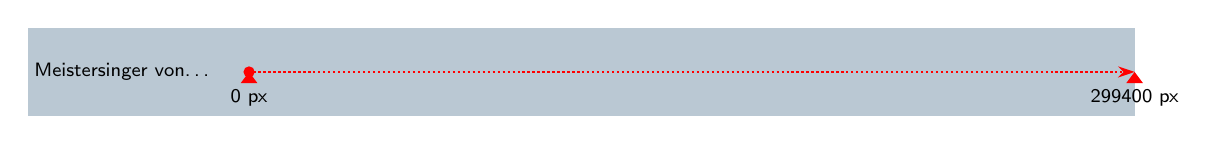
\begin{tikzpicture}[x=1pt,y=1pt,line width=0.8pt,inner sep=2pt,font=\sffamily\fontsize{7}{8.4}\selectfont]
\definecolor{ts000000}{HTML}{000000}
\definecolor{tsBAC8D3}{HTML}{BAC8D3}
\definecolor{tsFF0000}{HTML}{FF0000}
\fill[tsBAC8D3] (0,0) rectangle (400,32);
\draw[tsFF0000,densely dotted,{Circle[length=4pt]}-{Stealth[length=6pt,width=4pt,inset=2pt]},shorten <=-2pt] (80,16) -- (400,16);
\fill[tsFF0000] (80,16) -- (77,12) -- (83,12) -- cycle;
\fill[tsFF0000] (400,16) -- (397,12) -- (403,12) -- cycle;
\node[anchor=west,text=ts000000] at (0,16) {Meistersinger von…};
\node[anchor=north,text=ts000000] at (80,12) {0 px};
\node[anchor=north,text=ts000000] at (400,12) {299400 px};
\end{tikzpicture}
\end{document}
